\documentclass[tikz,border=4pt]{standalone}
\usepackage{tikz}
\usetikzlibrary{arrows.meta}
\begin{document}
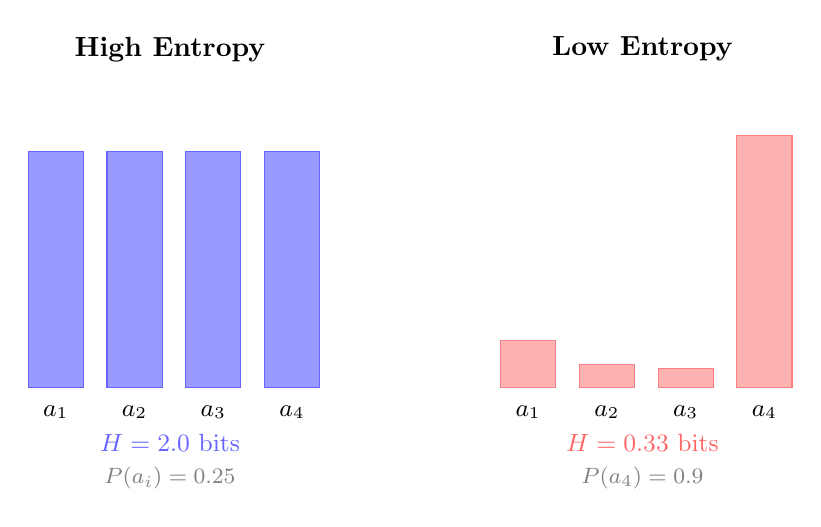
\begin{tikzpicture}[>=Stealth]
% === Left: high entropy ===
\begin{scope}[shift={(0,0)}]
    \node[font=\bfseries] at (2,4.3) {High Entropy};

    \foreach \i/\lbl in {0/$a_1$, 1/$a_2$, 2/$a_3$, 3/$a_4$} {
        \fill[blue!40,draw=blue!60] (0.2+\i*1,0) rectangle (0.9+\i*1,3);
        \node[font=\small,below] at (0.55+\i*1,-0.1) {\lbl};
    }

    \node[blue!60,font=\small] at (2,-0.7) {$H = 2.0$ bits};
    \node[gray,font=\footnotesize] at (2,-1.15) {$P(a_i) = 0.25$};
\end{scope}

% === Right: low entropy ===
\begin{scope}[shift={(6,0)}]
    \node[font=\bfseries] at (2,4.3) {Low Entropy};

    \fill[red!30,draw=red!50] (0.2,0) rectangle (0.9,0.6);
    \fill[red!30,draw=red!50] (1.2,0) rectangle (1.9,0.3);
    \fill[red!30,draw=red!50] (2.2,0) rectangle (2.9,0.25);
    \fill[red!30,draw=red!50] (3.2,0) rectangle (3.9,3.2);

    \foreach \i/\lbl in {0/$a_1$, 1/$a_2$, 2/$a_3$, 3/$a_4$} {
        \node[font=\small,below] at (0.55+\i*1,-0.1) {\lbl};
    }

    \node[red!60,font=\small] at (2,-0.7) {$H = 0.33$ bits};
    \node[gray,font=\footnotesize] at (2,-1.15) {$P(a_4) = 0.9$};
\end{scope}
\end{tikzpicture}
\end{document}
